\clearpage
\setcounter{page}{1}
\maketitlesupplementary
\renewcommand{\thesection}{S\arabic{section}}
\renewcommand{\thetable}{S\arabic{table}}
\renewcommand{\thefigure}{S\arabic{figure}}
\setcounter{section}{0}\setcounter{table}{0}\setcounter{figure}{0}
\noindent This supplement provides implementation details, cohort construction, inference procedures and additional analyses. Sections and tables prefixed with ``S'' refer to this document; all other numbers refer to the main paper. The low-texture LUNA16 subset of the main paper is referred to as the focused study.

\section{Exterior Forecast and Controls}
\label{supp:fit}
\paragraph{Spatial support.}
Each axial CT neighborhood is resampled onto a $64^3$ grid in slice, row and column order with spacing $1.5\times0.7\times0.7\mm$ and normalized intensity $(\mathrm{HU}+1000)/1400$. Signed values are retained for affine fitting, subtraction and the Hessian of the residual. The forecaster observes voxels at distances strictly greater than 14\,mm from the center, and the estimated field is tapered between 22 and 26\,mm. The search core has a radius of 10\,mm, and each window extends a further 6\,mm around its center.

\paragraph{Vessel field estimation.}
The masked crop is smoothed with a Gaussian of $0.85\mm$ standard deviation and normalized by the smoothed visibility mask, with a small floor on the denominator. Intensity and prominence are sampled at 2,400 nearly uniform anchors on the $15.5\mm$ sphere, and flank values are taken from neighboring anchors 2.6--3.8\,mm away. We retain up to 14 prominent peaks separated by at least $4.1\mm$ and pair peaks that are at least $27.3\mm$ apart. At each end of a chord, the continuation score is the axial intensity minus the mean of four transverse samples, evaluated at radii of 17.8 and 20.4\,mm. Up to three disjoint pairs with sufficient bilateral contrast are kept, with priority given to agreement between legs and proximity to the crop center.

Each leg is fitted to exterior samples within a transverse radius of $5.5\mm$ and at signed chord distances of 11--21\,mm, using a local flank median as background. The width is selected from $\{1.15,1.50,1.85,2.20,2.55,2.9\}\mm$ as the value that maximizes the reduction in residual sum of squares of a nonnegative Gaussian cross-section. A track requires a valid fit on both legs and an amplitude of at least 77\,HU. Amplitude and width are interpolated along the chord, the resulting track fields are summed, and a cubic smoothstep implements the taper. Crops without fitted tracks remain in every denominator.

\paragraph{Verification of the controls.}
The rotation is an exact quarter-turn about the center voxel. Because the in-plane spacings are equal, every scored voxel maps to a voxel at the same physical radius, and we confirm that the value multiset is preserved on the central 13-mm support of every new control. On the first crop of each held-out block, we rerun the forecaster after replacing the hidden region and verify that the field is unchanged. Finally, the complete visible exterior is compared bitwise for every rendered insertion/control pair.

\section{Readout and Baseline Details}
\label{supp:heads}
\paragraph{Window computations.}
Window terms are computed by FFT-based correlation with an orthogonal weighted affine basis and three mean-centered compact kernels. Let $D=\|u\|_W^2$, $C=\langle z,u\rangle_W$ and $G=(1+\rho)D$. The fixed-residual loss is $J_{\mathrm{fix}}=\|z\|_W^2-2C+D$, and completing the square in $g-1$ gives the penalized null loss $J_0=J_{\mathrm{fix}}-(C-D)^2/G$. After elimination of $g$, the profile readout uses the effective squared template norm $d_{\mathrm{prof}}=\|t\|_W^2-\langle u,t\rangle_W^2/G$, whereas the plug-in readout retains $\|t\|_W^2$; both share $J_0$ and the projection of $z-g_0u$ onto $t$. Setting $u=0$ recovers the CT-only score.

\paragraph{Hyperparameters.}
The three coupled settings are
\begin{align*}
(\rho,\tau,C_{\rm log})\in\{&(0.025,0.018,0.008),\\
&(0.15,0.033,0.08),\,(0.75,0.055,0.8)\},
\end{align*}
with the floor $\tau$ in normalized CT units. We use $10^{-9}$ as a lower bound on $G$ and 0.05 as a lower bound on the squared template norm of the profile readout. Fixed subtraction uses unit amplitude in all settings, since its tube amplitudes are already fitted on the exterior. The Hessian baseline uses the same signed field with subtraction strengths $0.35$, $0.7$ and $1.0$, followed by Gaussian derivative scales of 1.3, 2.5 and 4.0\,mm and an established compact-curvature and smoothing recipe. Full subtraction was selected on the focused data, and the broader development grid selects its strength independently.

\paragraph{Classifier features.}
The 12 shared CT summaries are the peak and center values of the smoothed Hessian response, the center intensity, the near-center mean intensity, the peak core intensity, the bright core fraction, the mean core and core--ring intensities, the mean core response, the near-center vesselness and peak response, and the core intensity standard deviation. We add three unnormalized template maxima from a single 13-mm affine projection and three normalized CT-only maxima from the shared local bank. The exterior summaries are the mean excess above 0.22 and the fraction above 0.42 in the 15.5--19.5\,mm annulus, together with the peak and mean forecast values within 13\,mm. The shell-only classifier uses these summaries alone, while each spatial classifier adds three forecast-conditioned template maxima. Training features are standardized on the fitting rows, each control is weighted equally with its entire bank of insertions, and all logistic classifiers use an intercept and an $\ell_2$ penalty.

For an empty forecast the spatial and local template measurements coincide before classification. Differences between classifiers can nevertheless arise through the four summary features, the additional template inputs and the fitted coefficients. The rotated spatial classifier controls for all of these channels, and the rotation evaluated with the aligned classifier applies identical coefficients and settings to both placements.

\section{Cohorts and Insertion Banks}
\label{supp:cohort}
\begin{table}[t]
\centering
% Cohort roles (moved from supplement Table S1; same numbers).
\setlength{\tabcolsep}{4pt}\footnotesize
\begin{tabular}{@{}lrrr@{}}
\toprule
Role & Blocks & Controls & Insertions \\
\midrule
Focused fit & 46 & 138 & 2,484 \\
Focused development & 39 & 117 & 2,106 \\
Focused calibration & 92 & 276 & -- \\
Focused evaluated & 183 & 549 & 9,882 \\
\midrule
Broader fit & 80 & 240 & 4,320 \\
Broader development & 85 & 255 & 4,590 \\
Broader calibration & 175 & 700 & -- \\
Broader holdout & 170 & 680 & 12,240 \\
\midrule
HiPaS development & 24 & 144 & 2,592 \\
HiPaS transfer & 72 & 432 & 7,776 \\
\bottomrule
\end{tabular}

\caption{\textbf{Cohort roles.} Blocks are LUNA16 patients or HiPaS scans. Each control contributes one negative decision and is paired with 18 insertions.}
\label{tab:roles}
\end{table}

\paragraph{LUNA16 rosters.}
The LUNA16 archive provides an auditable TCIA subject crosswalk and a separate list of irrelevant findings~\cite{setio2017,armato2011}. For the broader test and calibration rosters, we exclude every patient used in the original focused fitting, development, calibration, test or shift roles, the two broader fitting and development folds, and the subject repeated across folds. Within each remaining fold, a fixed permutation assigns patients to disjoint roles; the calibration roster retains 175 of 177 assigned patients and the test roster 170 of 174, with eligibility requiring four spatial neighborhoods. All source volumes were checksum-verified, and all sampling seeds and inclusion lists were fixed before test scoring.

\paragraph{Candidate sampling.}
Candidate centers are at least 38\,mm apart and more than 27\,mm from the boundary of any included or irrelevant finding. New crops require sufficient source support for the field fit, a parenchymal median in the inner region, and at most 12\% of the 26-mm support above $-552\hu$; the reused broader fitting and development caches applied a stricter occupancy limit of 5.5\%. Core texture is unrestricted in the new sample. Before insertion, the core SD of the broader held-out set spans 59--255\,HU between the 10th and 90th percentiles (median 117\,HU), and the corresponding HiPaS values are 123--407\,HU (median 253\,HU).

\paragraph{Lesion banks.}
The focused study used compact signals $(1-d^2/r^2)_+^{0.72}$ with radii of 1.85 and 3.35\,mm and contrasts of 70, 182 and 336\,HU. The broader study uses a bank based on the anisotropic component $L(p)=\exp(-u^2)(1-u^2)_+^{0.6}$, where $u$ is the ellipsoidal radius. The bilobed shape combines two translated components with weights 0.72 and 0.52, and the part-solid-like shape combines a broader halo and a smaller translated component with weights 0.40 and 0.60. A random rotation and axis stretch is shared across the bank of a crop, and each sampled peak is normalized to the prescribed contrast. Displacements of 0, 4 and 7\,mm relative to the candidate center are applied along a fixed random direction per background. All lesion-model choices were finalized on development data before the held-out set was scored.

\paragraph{Native-vessel transfer.}
HiPaS provides de-identified noncontrast CT with separate artery and vein masks~\cite{chu2025hipas}; we use release v2. The first 24 previously inspected scans serve as a development check. The 72 evaluation scans were drawn from the remaining release before any test scores were computed, and all staged volumes were checksum-verified. Six candidate neighborhoods per scan are sampled at midpoints between annotated artery and vein surfaces separated by 2.5--8\,mm, at least 24\,mm apart, with annotated foreground in the search core and a parenchymal median in the inner neighborhood. Lesion morphology and displacement are rendered independently of the forecast. The proximity stratum is defined by a minimum distance of at most 2\,mm between the lesion support and the vessel mask, and overlap is the fraction of the lesion support that intersects the mask. The release identifies scans but lacks a public crosswalk for repeat patients. The vascular background consists entirely of the original images.

\section{Inference and Operating Points}
\label{supp:inference}
\paragraph{Cutoffs.}
The matched operating point uses a strict rank cutoff with $k=\lfloor0.10N_0\rfloor$ admissible negative acceptances. Let $s_{(1)}\geq\dots\geq s_{(N_0)}$ denote the negative scores; a candidate is accepted when its score exceeds $s_{(k+1)}$. Test scores determine the cutoff of the within-test ROC, whereas independent LUNA16 negatives determine the frozen cutoff. Stratified comparisons retain the global, scorer-specific cutoffs. Localization additionally requires the highest normalized template peak to lie within 3\,mm of the insertion center, while the crop score remains the ridge output of the same scorer. A control counts against the FPR budget whenever it passes the crop cutoff.

\paragraph{Bootstrap.}
We draw 3,000 shared patient resamples within acquisition folds. The test ROC recomputes the order statistic with the drawn multiplicities and treats ties as a group. Frozen intervals are conditional on the realized calibration patients and thresholds, whereas recalibrated intervals use an independently seeded stratified bootstrap of the calibration patients. Test and calibration draws remain paired across scorers. The resulting sensitivity and FPR intervals are reported in Table~4 of the main paper, the ROC curves in Fig.~5, and the full HiPaS operating points in Table~3. The localization endpoint and the condition analyses are secondary, and their intervals are not adjusted for multiplicity.

\paragraph{Sample size and criteria.}
The development bootstrap used to plan the study estimated that approximately 123 patients provide 80\% power to detect a nonzero crop-sensitivity difference against the refitted rotation, and 74 patients against fixed subtraction, assuming a true improvement of 5\,pp and development-level variability on the holdout. The calculation scales the observed bootstrap standard deviation by $\sqrt{85}$ and uses the normal quantiles 1.96 and 0.842; the 170 eligible test patients exceed both requirements. The practical criterion additionally required an observed point estimate of at least 5\,pp in both comparisons, and the frozen criterion required an FPR of at most 13\% and an upper limit of at most 4\,pp on the paired excess FPR. The broader test did not meet the prespecified crop-level criteria.

\begin{table*}[!t]
\centering
\small
\begin{tabular}{@{}lrlrl@{}}
\toprule
& \multicolumn{2}{c}{Focused fixed $-$ rotation} & \multicolumn{2}{c}{Broader profile $-$ rotation} \\
\cmidrule(lr){2-3}\cmidrule(lr){4-5}
Insertion group & $n$ & Sensitivity $\Delta$ (95\% CI) & $n$ & Sensitivity $\Delta$ (95\% CI) \\
\midrule
Centered & 3,294 & -0.94 [-5.98, +2.07] & 4,080 & -5.34 [-9.49, -1.25] \\
Displaced & 6,588 & +22.56 [+19.22, +24.83] & 8,160 & +5.80 [+4.02, +7.65] \\
Faintest & 3,294 & +0.70 [-2.00, +2.34] & 4,080 & -1.47 [-2.60, -0.24] \\
Strongest & 3,294 & +27.32 [+24.29, +30.15] & 4,080 & +7.92 [+4.26, +11.72] \\
Strongest, displaced & 2,196 & +42.53 [+38.39, +46.18] & 2,720 & +15.40 [+11.84, +19.08] \\
Overlap $\geq 50\%$ & 6,900 & +9.52 [+5.29, +12.20] & 5,991 & -0.12 [-3.59, +3.23] \\
\bottomrule
\end{tabular}

\caption{\textbf{Paired crop-sensitivity changes at the global matched FPR cap.} Strata may overlap. Faintest and strongest denote the extreme contrasts within the respective bank. The focused analysis uses fixed subtraction with settings selected on the focused development data; the broader analysis uses the preselected profile.}
\label{tab:strata}
\end{table*}

\section{Localization and Conditional Analyses}
\label{supp:loc}
\paragraph{Location transitions.}
Localization can improve without a change in the crop decision. At the broader matched cap, the refitted rotation of the profile accepted 1,699 lesion crops with an off-target location and localized 900, whereas the aligned profile localized 1,646. Table~\ref{tab:transitions} cross-tabulates the paired decisions. Alignment moved 386 accepted off-target locations to within 3\,mm and 124 in the opposite direction; it further localized 647 crops rejected by the rotation and lost 163 localized crops to rejection, for a net gain of 746 localized insertions. The corresponding analysis on native-vessel backgrounds yields 284 newly localized and 69 lost insertions.

\begin{table}[t]
\centering
\small
\begin{tabular}{@{}lrrr@{}}
\toprule
 & \multicolumn{3}{c}{Aligned profile} \\
\cmidrule(lr){2-4}
Refitted rotation & Rejected & Off target & Within 3 mm \\
\midrule
Rejected & 8,599 & 395 & 647 \\
Off target & 624 & 689 & 386 \\
Within 3 mm & 163 & 124 & 613 \\
\bottomrule
\end{tabular}
\caption{\textbf{Location transitions on the broader held-out set.} Counts are over the same 12,240 lesion crops at each scorer's overall 10\% candidate FPR cutoff; the diagonal contains unchanged decisions.}
\label{tab:transitions}
\end{table}

\paragraph{Alternative comparisons.}
Fixed subtraction, the strongest alternative readout, was selected as a comparator for the lead scorer. Compared with its own separately tuned rotation, it yields localized gains of $+9.66\pp$ $[+8.24,+11.38]$ on the broader held-out set and $+2.39\pp$ $[+1.22,+3.28]$ on HiPaS. This post hoc analysis uses the locked scores, whereas the primary placement comparison uses the preselected profile. Evaluating the rotation with the aligned classifier gives localized differences of $+4.26\pp$ $[+2.39,+5.83]$ on the broader held-out set and $+0.51\pp$ $[-0.15,+1.09]$ on HiPaS.

\paragraph{Forecast dominance.}
The dominance score is the peak forecast within 13\,mm divided by 0.02 plus the 80th--20th percentile spread of the exterior residual in the 15.5--19.5\,mm annulus, split at the median of the broader development data. On the broader held-out set, the high-dominance band contains 277 controls and 4,986 insertions. Within this band the aligned and rotated profiles have frozen FPRs of 11.19\% and 9.39\% and miss 3,731 and 4,009 insertions; outside it, the corresponding values are 10.17\% and 8.44\% with 5,597 and 5,870 misses. The score serves as a descriptive measure of forecast strength relative to exterior texture, and all cases are retained in the analysis.

\section{Learned Baseline and Computational Cost}
\label{supp:learned}
\paragraph{Architecture and training.}
The hybrid scorer operates on $25^3$ voxels at 1.35-mm spacing, cropped from the resampled observed image and the auxiliary volume. Its convolutional layers have 10, 12 and 8 channels with kernel widths of 5, 3 and 1 and an initial stride of 2. Each channel is summarized by the mean of its eight largest activations in the search core and by its mean within 4.5\,mm. The resulting 16 learned features and 18 shared CT summaries feed a nonlinear classifier with 20 hidden units, complemented by a trainable linear CT path. The network is trained from scratch on the focused fitting data without an external encoder. The auxiliary channel contains average-pooled CT for the CT-only network, the aligned or rotated field for the forecast networks, and the signed residual alongside the unchanged CT channel for the residual network.

All four networks use the same sampled insertion variants, axial rotations and slice reflections, AdamW with an initial learning rate of 0.003 and cosine decay, two seeds, and snapshots at 10, 20 and 30 epochs. The snapshot is selected by development sensitivity at the matched cap, and the logits of the two seeds are averaged. As a sanity check, the CT-only network reaches 99.48\% training AUROC on 12 control crops and 48 strong off-center lesions from four fitting patients, and 86.42\% on a harder probe of the same size containing all insertion variants. Trained on all 46 fitting patients, it comes within one point of the local ridge classifier on development in both AUROC and sensitivity. Fig.~\ref{fig:learned} shows the learning curve and both fitting checks; the comparison on the focused cases is reported in Table~2 of the main paper.

\begin{figure*}[t]
\centering
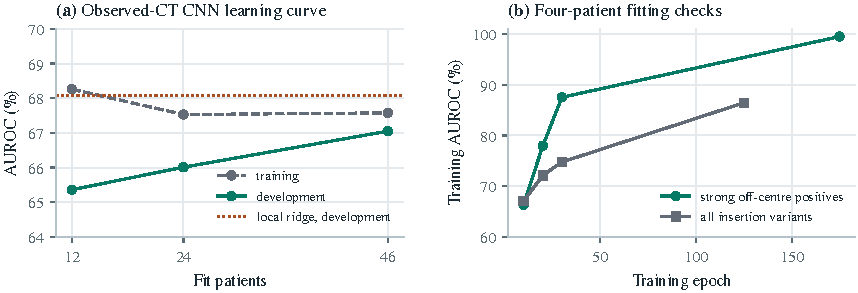
\includegraphics[width=\textwidth]{figures/learning.pdf}
\caption{\textbf{Training behavior of the CT-only CNN.} (a)~AUROC versus the number of fitting patients (single-seed snapshots; the reported 67.54\% averages two seeds), with the ridge classifier on development for reference. (b)~Training AUROC on four fitting patients for an easy setting (strong off-center lesions) and a hard setting (all insertion variants), the latter recorded up to 125 epochs.}
\label{fig:learned}
\end{figure*}

\paragraph{Selective use and cost.}
For each extrapolated chord we compare the predicted and observed center-to-flank contrast beyond the amplitude-fit support on both legs. The resulting reliability score uses the weaker signed support and penalizes contrast disagreement; the selective policy ranks crops by this score and otherwise falls back to the shell-only classifier. A control policy ranks crops by peak forecast strength instead. Both use the same three development coverage budgets and the same scores for each branch. At approximately 65\% coverage, the two policies reached 48.91\% and 47.91\% sensitivity, compared with 52.14\% for always using aligned fixed subtraction, all at the same negative cap.

Run time was measured on a single CPU thread over 120 loaded crops from 30 focused development patients, with method order randomized. The timed path comprises a new forecast, the decision branch, feature computation, the full search and the classifier for each candidate; for the two policies it additionally includes the reliability or strength score. The selective and strength-based policies required 137 and 132\,ms per loaded crop, and always using the aligned fixed subtraction 133\,ms. The measurement excludes proposal generation and any clinical cost. The selective policy was evaluated on development data only and is not part of the fresh evaluation.

\section{Transfer Results of the Focused Design}
\label{supp:previous}
The focused study used separate thresholds derived from 276 controls. It supported a substantial placement effect, but its upper limit on the excess FPR relative to the CT-only classifier was 4.92\,pp, above the stipulated 4\,pp. The morphology-shift condition and the independent LNDb acquisition with shifted insertions did not meet the full transfer criteria~\cite{pedrosa2021}; their achieved rates are listed in Table~5 of the main paper. Within each test set, the profile and Hessian sensitivities at 10\% FPR were 37.93\% and 37.44\% under the morphology shift and 33.15\% and 32.94\% on LNDb, illustrating the distinction between ranking and calibration transfer.

The LNDb detector analysis used the scores and boxes of the Duke detector; adding the spatial features changed mean FROC by $0.00\pp$ $[-0.21,+0.23]$ relative to the full CT-only classifier and by $-0.13\pp$ $[-0.33,+0.35]$ relative to the corresponding sham. The controlled HiPaS transfer addresses a different question, namely localized detection of inserted targets on annotated vascular backgrounds.
